\documentclass{article}
  % Packages and package settings
  \usepackage{fontspec}
    \setmainfont{Charis SIL}
  \usepackage{hyperref}
    \hypersetup{colorlinks=true,
                allcolors=blue}
  \usepackage{graphicx}
    \graphicspath{{./figures/}}
  \usepackage{phonrule}

  % Title info
  \author{Joshua McNeill}
  \title{Homework 2}
  \date{\today}

  % Custom commands
  \newcommand{\lexi}[1]{\textit{#1}}

\begin{document}
  \maketitle
  \begin{enumerate}
    \item (Lab 2 Step 10)

    There is clearly some structured positional variation in the duration of vowels in English. Zsiga explains that ``[v]owels are lengthened in open syllables, and before consonants'' (p.~70), which does in fact appear to be what is happening in our data. To begin with, Figure \ref{fig:durVowel} shows that different vowels have different duration in general: [ɑ], [i], and [u] are on the shorter side and the diphthongs as well as [ɔ] are on the longer side. It is also apparent in Figure \ref{fig:durStructure} that the structure of the syllable, whether it is open (i.e., CV) or closed (i.e., CVC), has an impact on vowel duration, with vowels in open syllables being longer. However, Figure \ref{fig:durFinalC} shows that it is not just whether the syllable is open or closed, but also whether the final consonant is /t/ or /d/, where /d/ leads to vowel durations similar to those of open syllables. Finally, to clarify that this is not simply confounding with certain vowels being in certain syllable structures, Figure \ref{fig:durVC} gives the conditional distribution for vowel durations by final consonant for each vowel. The result confirms that vowel duration really is longer in open syllables and when the final consonant is voiced, at least with final /d/ compared to final /t/. The rule might be stated in the following way:
    \begin{enumerate}
      \item \phonc{V}{\phonfeat{+long}}{\oneof{\phold \phonfeat{+voiced} \\ \phold \#}}
    \end{enumerate}
    
    \begin{figure}[htb]
      \caption{Mean vowel duration (seconds) by vowel}
      \label{fig:durVowel}
      \centering
      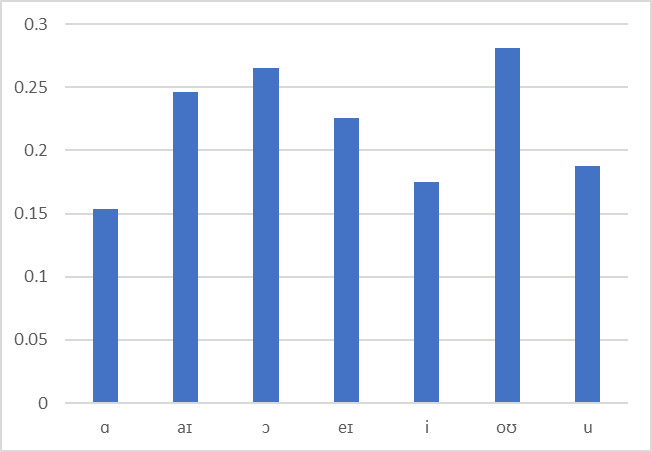
\includegraphics{durVowel.jpg}
    \end{figure}

    \begin{figure}[htb]
      \caption{Mean vowel duration (seconds) by syllable structure}
      \label{fig:durStructure}
      \centering
      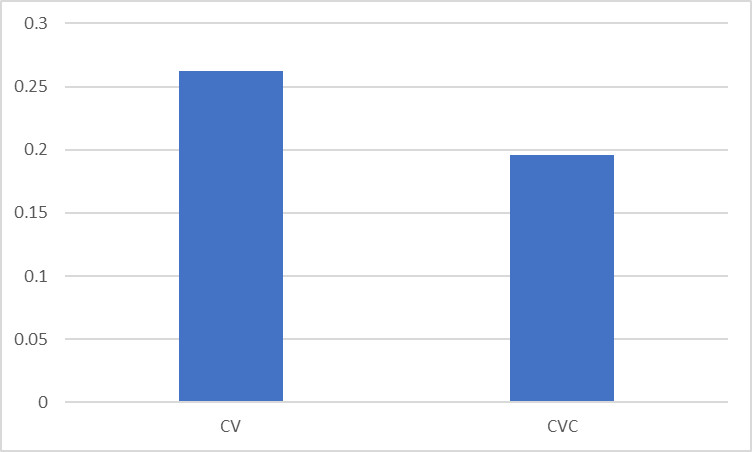
\includegraphics{durStructure.jpg}
    \end{figure}

    \begin{figure}[htb]
      \caption{Mean vowel duration (seconds) by final consonant}
      \label{fig:durFinalC}
      \centering
      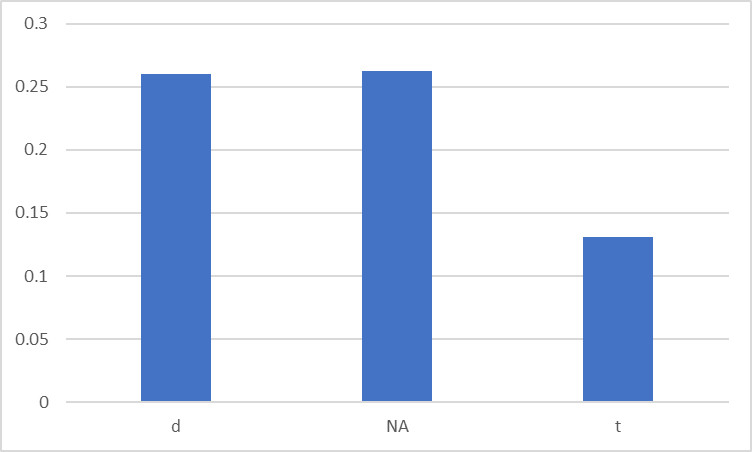
\includegraphics{durFinalC.jpg}
    \end{figure}

    \begin{figure}[htb]
      \caption{Mean vowel duration (seconds) by vowel and final consonant}
      \label{fig:durVC}
      \centering
      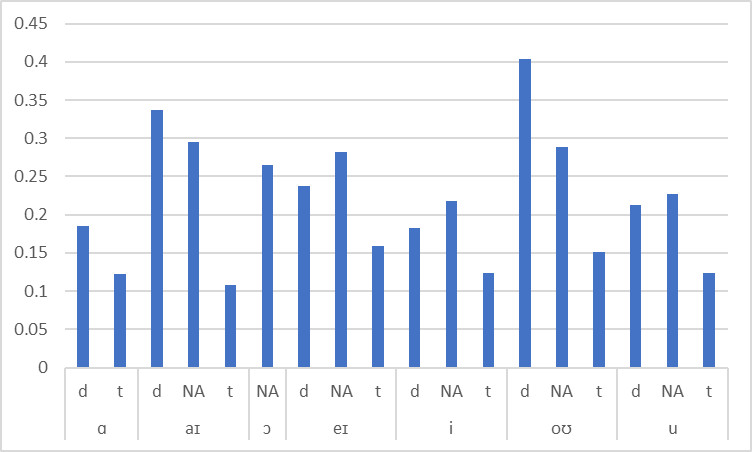
\includegraphics{durVC.jpg}
    \end{figure}
    \item Transcription:

    [aɪ lʊkt ʌp ən sɔ ðæt̚ ðɛɹ wəz ə pʰəlismən stæ̃ndɪ̃n ɪ̃n fɹʌ̃n ə mi ɛ̃n i wəz seɪən ɛ̃niwən æt̚ hoʊm bəɾ aɪ dɪən noʊ wʌt̚ ðæt̚ mɛ̃nt̚ ɛ̃n ðɛ̃n i sɛd ɑɹ ju̟ ɑl ɹaɪt̚ jʌ̃ŋ mæ̝̃n aɪ lʊkt æɾ əm ən aɪ θɔt̚ fəɹ ə bɪt̚ soʊ ðæɾ aɪ wʊd̚ æ̝̃ntsəɹ ðə kwɛʃtʃən kʰəɹɛkli ɛ̃n aɪ sɛd noʊ ɛ̃n i sɛd jəɹ lʊkɪ̃n ə bɪt̚ wərs fəɹ wɛɹ i æd ə ɡɔld̚ ɹɪ̃ŋ ɔ̃n wʌ̃n əv ɪz fɪ̃ŋɡəɹs ɛ̃n ɪt̚ hæd kʰəɹli lɛɾəɹz ɔ̃n ɪt̚ bəɾ aɪ kʰʊd̚n si wʌt̪̚ ðə leɾəɹz wəɹ ðɛ̃n i sɛd̚ ðə leɪɾi æt̪̚ ðə kʰæfeɪ sɛz ju̟v bɪ̃n iɹ fəɹ tʰu̟ ən ə hæf aʊɹz ɛ̃n wɛ̃n ʃi t̠ɹaɪd̚ tʰɔkɪ̃n tʰə jə, ju̟ wəɹ ɪ̃n ə kʰəmpʰlit̠̚ t̠ɹæ̝̃nts ðɛ̃n i sɛd wʌtʃ jəɹ neɪ̃m ɛ̃n aɪ sɛd kɹɪstəfəɹ bu̟n ɛn i sɛd wɛɹ ɾə jə lɪv ɛ̃n aɪ sɛd θʌɾi sɪks ɹæ̝̃ndɔf s̠t̠ɹit̚ ɛ̃nd aɪ stɑɹɾɪd filɪn bɛɾəɹ bikʰʌz aɪ laɪk pʰəlismən ɛ̃n ɪt̚ wəz ən izi kwɛʃtʃən]

    There were several passages in the above transcription that were phonologically interesting. Word-final alveolar stops in words such as \lexi{thought} were rarely released. In this case, the following word \lexi{for} began with a consonant, but even in a series of words like \lexi{meant and}, the /t/ was realized as [t̚]. Some of these cases led to the tap [ɾ] being used if that sound was intervocalic, such as in \lexi{so that I would}, transcribed as [soʊ ðæɾ aɪ wʊd̚], with an [ɾ] at the end of \lexi{that}.

    The /t/s in words like \lexi{tried} and \lexi{trance}, where followed by /ɹ/, were also at least retracted to post-alveolar positions, though it is possible that they were fully affricated as [tʃ]. This occurred even if the cluster was preceded by /s/ as in \lexi{street}, which also had a retracted [s̠] that for some reason was clearly different from the non-retracted /s/ in \lexi{started}.

    In unstressed syllables, /ə/ and /ɪ/ were often not distinct, as in the \lexi{-ed} of \lexi{started}. In some words, this was particularly hard to transcribe, as in \lexi{saying}, which I transcribed as [seɪən]. In reality, it seems equally likely that the transcription could have been [seɪɪn] or [seɪn̩]. On a related note, \lexi{-ing} words were basically always pronounced with voiced alveolar nasals instead of velar, hence \lexi{saying} was not [seɪŋ].

    Words like \lexi{trance} and \lexi{answer} were very difficult to pronounce without an epenthesized [t] between the /n/ and /s/. However, this was not an issue at the word boundary in \lexi{couldn't see}, transcribed as [kʰʊd̚n si]. It is difficlt to know if this is due to the word boundary itself or the /t/ deletion.

    There was also an unexpected aspiration in the /p/ in the word \lexi{complete}, realized as [kʰəmpʰlit̠̚]. It makes sense in that /l/ is fairly sonorant, but it was unexpected nonetheless. Compared to the aspiration in \lexi{pit} and the lack of aspiration in \lexi{spit}, it was somewhere in between.

    Finally, both tokens of \lexi{question} were pronounced with [ʃtʃ], as in [kwɛʃtʃən]. From what I understand, for some speakers, this is a very unusual combination of sounds.
  \end{enumerate}
\end{document}
